\section{Post Production}
\subsection{Aufnahmeformate}
Bei der Auswahl des Aufnahmeformates muss man sich im Klaren sein, mit welchem Codec man aufnehmen möchte. Hierbei muss man zwischen Codecs und Containern unterscheiden. Container, welche den Videostream mittels eines Codecs digitalisieren, speichern die Videodaten auf dem Speicherchip. Audio Video Interleave (AVI), QuickTime (MOV) oder Moving Pictures Expert Groups (MPEG) sind zum Beispiel solche Containerformate. Ein Codec wandelt analoge Bilder in digitale Datenströme um. Bei der Codierung wird das Bild komprimiert, was wiederum mehr Speicherplatz zur Verfügung stellt. DivX, QuickTime H.264, Apple ProRes, Panasonic AVC-Intra oder Avid DNxHD sind typische Codecs.\footnote{vgl. Jörg Jovy, 2017, S. 114f.}\newline
Die Komprimierung des Videosignals erfolgte bei allen vier Videos mittels dem H.264 Codec im QuickTime (MOV) Container. 
\paragraph{MPEG}
\leavevmode \\
"MPEG ist ein standardisiertes Kompressionsverfahren, das sich speziell zur Datenreduktion von Bewegtbildern eignet." (https://www.film-tv-video.de/term-word/mpeg/ [Zugriff: 26.03.2018]) MPEG lässt dem Gerätehersteller freie Wahl, bezüglich der Entscheidung der Datenerzeugung. Jedoch legt MPEG das Datenformat und die Dekodierung vor. Was noch beachtet werden muss, ist, dass schlussendlich ein normgerechter MPEG-kodierter Datenstrom entstehen muss, der mit einem MPEG-Decoder gelesen und wiedergegeben werden kann. Bei dem MPEG Standard setzen sich die Einzelbilder einer Videosequenz aus einer Folge von I-, B- und P-Frames zusammen. Diese Aufeinanderfolgung wird Group of Pictures, kurz GOP, genannt. Eine Group of Pictures muss mindestens ein I-Frame enthalten. I-Frames sind Indexbilder, welche die wichtigsten Bildinformationen enthalten. "B-Frames sind  bidirektionale Bilder, also Frames, die nur die Unterschiede eines Bildes zum vorhergehenden oder folgenden Bild beinhalten." (https://www.film-tv-video.de/term-word/mpeg/ [Zugriff: 26.03.2018]) P-Frames sind Predicted Frames. Predicted Frames werden aus den vorherigen I-Frames berechnet.\newline
\begin{figure}[H]
	\centering
	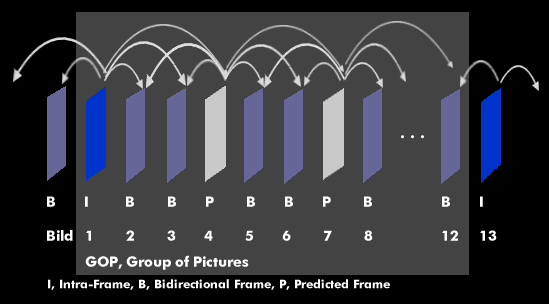
\includegraphics[width=0.8\textwidth]{abb27} 
	\caption[Group of Pictures]{Group of Pictures\footnotemark}
\end{figure}
\footnotetext{Quelle: https://www.itwissen.info/GOP-group-of-picture.html}
Der QuickTime Container ist im Grunde, wie das MPEG Containerformat aufgebaut. Jedoch ist QuickTime ein eigenes Containerformat von Apple.\footnote{vgl. https://www.film-tv-video.de/term-word/mpeg/ [Zugriff: 26.03.2018]}
\subsection{Kompressionsverfahren}
Bei der Bildkompression werden die Bildinformationen in 4x4, 8x8 oder 16x16 Pixeln zusammengefasst. "In einzelnen Bildern und zwischen aufeinanderfolgenden Bildern werden dann sich wiederholende Daten identifiziert." (Jörg Jovy, 2017, S. 117)\newline
Nun können die wiederholenden Informationen gefiltert und weggelassen werden. Bei dem MPEG-2 Container wird zum Beispiel nur jedes zwölfte Bild komplett gespeichert, wobei bei den anderen Bildern nur Teile beziehungsweise Veränderungen gespeichert werden. Da nur jedes zwölfte Bild komplett gespeichert wird, ist das Risiko enorm groß, dass Artefakte, also Bildfehler, entstehen können. Die sogenannten Artefakte entstehen bei der Umwandlung von digitalen Bildern in analoge Bildsignale.\footnote{vgl. Jörg Jovy, 2017, S. 117}
\subsection{Schnittprogramme}
\paragraph{Lightworks}
\leavevmode \\
Lightworks ist ein lizenzfreies Videoschnittprogramm, das auf Windows, Linux und auf IOS Betriebssystemen verwendet werden kann. Lightworks bietet nicht nur die freie Version, sondern auch eine Pro Version. Die freie Version bietet dem User eine Vielzahl an importierbaren Formaten, wie zum Beispiel Apple Pro Res, AVC-Intra 50, MPEG-2 Long GOP und vieles mehr. Weiters kann man in Lightworks seine Videos mit dem Codec H.264 mit der Auflösung 1280x720p kodieren.\footnote{vgl. Jörg Jovy, 2017, S. 355}\footnote{vgl. https://www.lwks.com/index.php?option\=com\_content\&view\=article\&id\=102\&Itemid\=213 [Zugriff: 02.04.2018]}
\paragraph{Adobe Premiere Pro}
\leavevmode \\
Adobe Premiere Pro ist eine kostenpflichtige Software, welche aber eine Vielzahl von Funktionalitäten bietet. Im Gegensatz zu Lightworks bietet Adobe Premiere Pro eine freie Auswahl, welche Formate man importieren möchte. Weiters bietet Premiere Pro eine umfangreiche Dokumentation. Zusätzlich sind Adobe Programme ähnlich aufgebaut und sind so einfach miteinander zu verknüpfen, wie zum Beispiel Premiere Pro mit Adobe After Effects.\footnote{vgl. Jörg Jovy, 2017, S. 358f.}
\subsection{Schnitt}
Bevor mit dem Schnitt begonnen werden kann, muss zunächst das Projektformat festgelegt werden. Bei Erstellung einer neuen Sequenz können folgende Parameter eingestellt werden
\begin{itemize}
	\item Bilder pro Sekunde
	\item Pixel - Seitenverhältnis
	\item Audio-Samplerate
	\item Bildgröße in Pixeln
	\item Render-Qualität
\end{itemize}
Hat man diese Eigenschaften festgelegt, kann man auch schon mit dem Schnitt beginnen. Es gibt drei Arten des Filmschnitts. Den Rough Cut oder schnelle Schnitt, 3-Punkt-Schnitt oder der exakte Schnitt und den 4-Punkt-Schnitt oder Zeitinterpolation.\footnote{vgl. Jörg Jovy, 2017, S. 384ff., S. 422ff.}
\subsection{Blenden}
Blenden signalisieren dem Zuschauer, dass es sich um eine neue Szene handelt. Blenden sind ein wertvolles Mittel, um den Film oder das Video angenehmer zum Ansehen machen. In Adobe Premiere gibt es eine Vielzahl an unterschiedlichen Blenden, bei denen man sich vorher überlegen sollte, was man mit der Blende bewirken will. In Premiere gibt es nicht nur typische Blenden, wie "Weiche Blende" oder "Filmblende", sondern auch Effektblenden. Die meisten Effektblenden werden jedoch nicht eingesetzt, da sie den Zuschauer nicht besonders ansprechen. Die einzige Effektblende, die verwendet wird, ist die Wipe oder auch Schiebeblende genannt.\footnote{vgl. Jörg Jovy, 2017, S. 438ff.}\newline
Bei dem Schnitt des Tag der offenen Tür Videos kam eine Blende zum Einsatz, nämlich die "Weiche Blende". Die weiche Blende wurde für die Übergänge verwendet von einer Frage zu der Antwort oder zum Ausblenden eines Textes.\newline
Bei dem Schnitt des Videos mit dem Absolventen kamen drei verschiedene Blenden zum Einsatz:
\begin{itemize}
	\item Wegschieben
	\item Filmblende
	\item Einzoomen \& Auszoomen
\end{itemize}
Die Wegschieben Blende ist sozusagen die Hauptblende und dient dazu, von einer einer Szene zur nächsten überzugehen. Die Filmblende blendet die erzielten Punkte ein und die Ein- und Auszommen Blende wurde für das Einblenden der Antworten genutzt.
\subsection{Color Correction}
Mithilfe der Lumetri-Scopes und der Farbkorrektur in Premiere Pro kann man die Farbe im Bild korrigieren. Einerseits gibt es die Lumetri-Scopes, bei denen man auf einen Blick erkennen kann, welche Farbinformationen nicht so dominant sind, ob das Bild über- oder unterbelichtet ist und wie die Helligkeitsverteilung im Bild ist. Und zum anderen gibt es die Farbkorrektur "Lumetri-Farbe" mit der man die oben genannten Eigenschaften verbessern kann.\footnote{vgl. Jörg Jovy, 2017, S. 520ff.}
\paragraph{Vektorskop}
\leavevmode \\
"Das Vektorskop gibt Auskunft über die Farbverteilung im Bild." (Jörg Jovy, 2017, S. 523) Auf dem Vektorskop sind die Grundfarben aus dem RGB und dem CMYK Farbraum abgebildet. Also: Rot, Grün, Blau, Cyan, Magenta, Yellow. Je weiter der Signalpunkt sich vom Zentrum entfernt, desto höher ist die jeweilige Farbsättigung. Hätte man ein Schwarz-Weiß-Bild würde man einen Punkt in der Mitte sehen.\footnote{vgl. Jörg Jovy, 2017, S. 523}\newline
Wie man auf der Abbildung \ref{fig:abb22} sehen kann, hat das Bild eine hohe Farbsättigung von Yellow und Rot, wohingegen es nur wenige Blauanteile hat.
\begin{figure}[H]
	\centering
	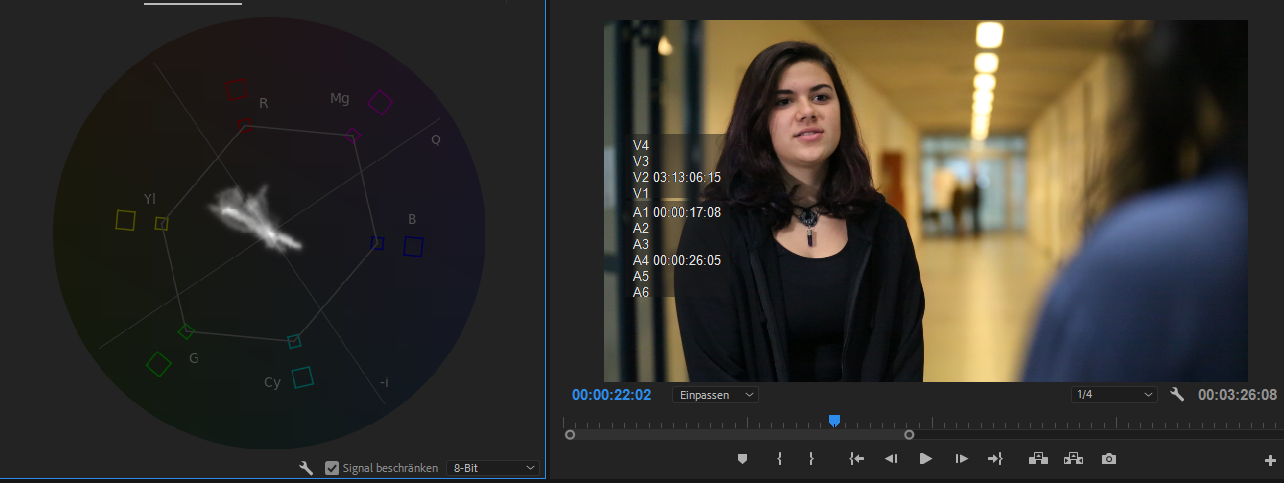
\includegraphics[width=1.0\textwidth]{abb22} 
	\caption{Vektorskop}\label{fig:abb22}
\end{figure}
\paragraph{Histogramm}
\leavevmode \\
Das Histogramm zeigt die Häufigkeitsverteilung von Helligkeit und Farbe, die im Bild vorkommt. Weiters zeigt das Histogramm, ob das Bild korrekt belichtet wurde. Das Histogramm geht von 0,0,0 für RGB Schwarz bis 255,255,255 für RGB Weiß. Die Schatten befinden sich beim Histogramm unten, also in Richtung 0,0,0, wobei man die Lichter oben, also in Richtung 255,255,255 findet.\footnote{vgl. Jörg Jovy, 2017, S. 523f.}\newline
Bei dem Histogramm sieht man, wie bei dem Vektorskop, dass die Farben Yellow und Rot eindeutig dominieren. 
\begin{figure}[H]
	\centering
	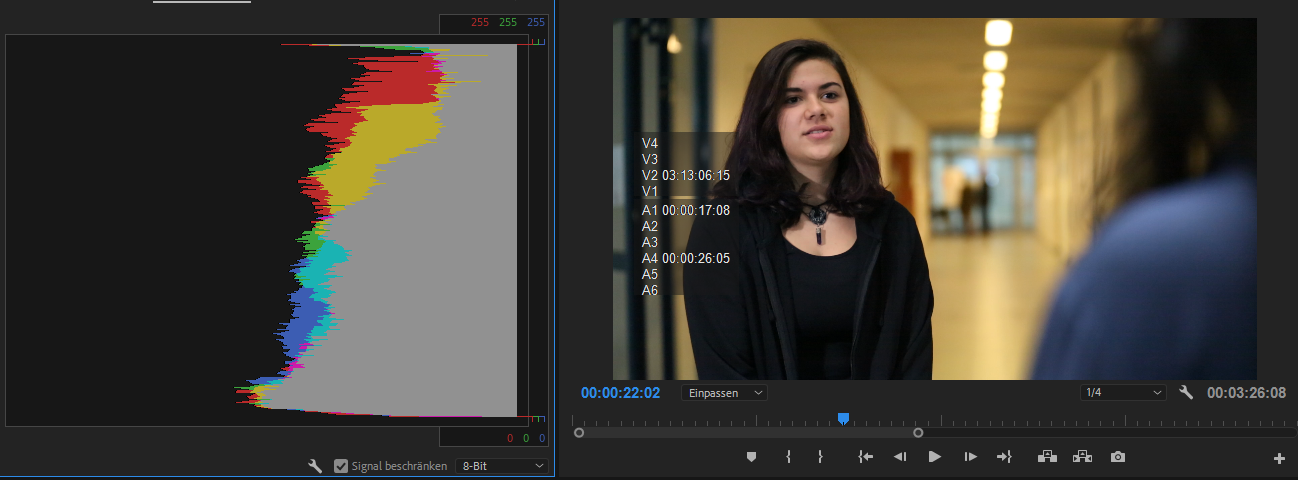
\includegraphics[width=1.0\textwidth]{abb21} 
	\caption{Histogramm}
\end{figure}
\paragraph{Waveform-Monitor}
\leavevmode \\
Der Waveform-Monitor zeigt die Helligkeitsverteilung im Bild. Die Helligkeit wird als Häufigkeitsverteilung wiedergegeben, wobei 100\% Weiß einen Messwert von 100 IRE entsprechen. "IRE ist die international übliche Skalierung." (Jörg Jovy, 2017, S. 522)\newline
0 IRE entsprechen daher Schwarz. Mithilfe des Waveform-Monitors kann man die sogenannten Lichter, Mitten und Tiefen einfach analysieren.\footnote{vgl. Jörg Jovy, 2017, S. 522ff.}\newline
Wie man auf der Abbildung \ref{fig:abb20} sehen kann, reichen die Tiefen bis zu dem Null Wert, das heißt es werden auch die Schatten völlig ausgeschöpft. Die Mitten sollten zwischen 50 und 70\% liegen und befinden sich auch, wie man hier sehen kann, in dem Bereich.\footnote{vgl. Jörg Jovy, 2017, S. 525}
\begin{figure}[H]
	\centering
	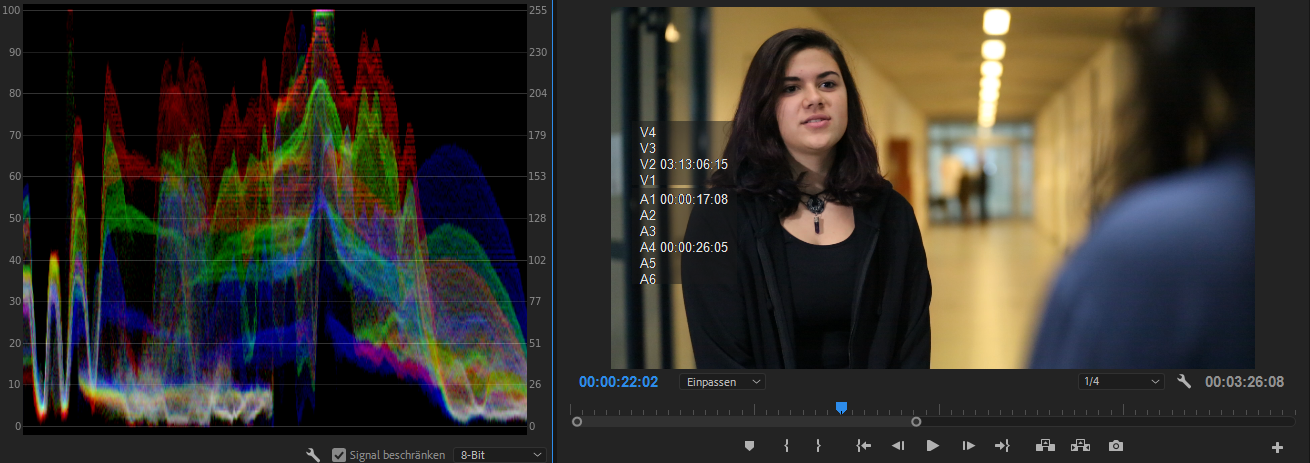
\includegraphics[width=1.0\textwidth]{abb20} 
	\caption{Waveform-Monitor}\label{fig:abb20}
\end{figure}
\subsection{Lumetri-Farbkorrektur}
\paragraph{Einfache Korrektur}
\leavevmode \\
Bei der einfachen Korrektur können grundlegende Verbesserungen vorgenommen werden:\footnote{vgl. https://helpx.adobe.com/at/premiere-pro/using/color-workflows.html [Zugriff: 31.03.2018]}
\begin{itemize}
	\item Weißabgleich
	\item Farbton
	\item Sättigung
\end{itemize}
\paragraph{Kreativ}
\leavevmode \\
Im Kreativ-Bereich kann dem Video ein bestimmter Look verpasst werden, wie zum Beispiel ein CineSpace Look. Weiters kann der Scharfzeichner, die Dynamik und die Sättigung eingestellt werden.\footnote{vgl. https://helpx.adobe.com/at/premiere-pro/using/color-workflows.html [Zugriff: 31.03.2018]}
\paragraph{Kurven}
\leavevmode \\
Bei den Kurven kann man zwischen RGB-Kurven und Farbtonsättigungskurven unterscheiden.\newline
Mit den RGB-Kurven kann die Luminanz und die Farbtonbereiche des Bildes angepasst werden. Man kann die Kurve entweder für alle drei RGB-Kanäle gleichzeitig anpassen, oder man kann es auch für die einzelnen RGB-Farbkanäle anpassen, also für Rot, Grün und Blau.\newline
Bei der Farbtonsättigungskurve kann die Sättigung angepasst werden. Man kann die Sättigung bestimmter Farbtöne verringern und erhöhen.\footnote{vgl. https://helpx.adobe.com/at/premiere-pro/using/color-workflows.html [Zugriff: 31.03.2018]}\newline
Wie man anhand der Abbildung \ref{fig:abb19} sehen kann, ist, dass die rote Farbtonsättigung erhöht wurde. Dies hatte diesen Effekt, dass die Gesichtsfarbe der Person in einen rötlicheren Farbton veränderte.
\begin{figure}[H]
	\centering
	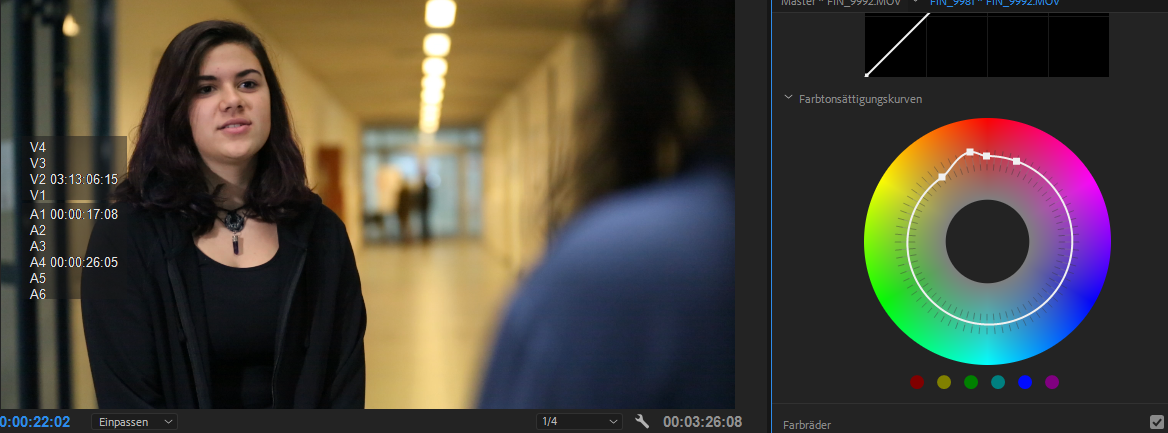
\includegraphics[width=1.0\textwidth]{abb19} 
	\caption{Farbtonsättigungskurve}\label{fig:abb19}
\end{figure}
\paragraph{Farbräder}
\leavevmode \\
Bei den Farbrädern können die Schatten, Mitteltöne und Glanzlichter angepasst werden.\footnote{vgl. https://helpx.adobe.com/at/premiere-pro/using/color-workflows.html [Zugriff: 31.03.2018]}
\subsection{Masken}
In Adobe Premiere Pro kann man mit Masken einen bestimmten Bereich markieren, den man anschließend verändern möchte. In der folgenden Abbildung \ref{fig:abb28} kann man die Verwendung der Maske von dem Interview mit dem Abteilungsvorstand sehen. 
Hierbei wurde die Maske mit einem Weichzeichner versehen, um den Hintergrund unscharf wirken zu lassen. Die Masken können mit einem Ellipsen-Werkzeug, Rechteck-Werkzeug oder einem Zeichenstift erstellt werden. Für die abgebildete Maske kam der Zeichenstift in Verwendung. Nach dem die Maske gezeichnet wsurde, kann man die Maske frame für frame bewegen. In diesem Fall konnte sich die Maske nicht automatisch mitbewegen, da sich der Hintergrund von der Maske nicht abgehoben hat. Somit musste die Maske manuell nachbearbeitet werden.\newline
Um einen flüssigen Übergang zwischen dem Maskenauswahlrahmen und dem Bereich außerhalb der Auswahl zu erzeugen, kann man eine weiche Kante anwenden.\footnote{vgl. https://helpx.adobe.com/de/premiere-pro/using/masking-tracking.html [Zugriff: 31.03.2018]}\begin{quote}Die weichen Kanten glätten den Maskenauswahlrahmen, sodass die Maske mit dem Bereich außerhalb der Auswahl verschmilzt und ein ästhetisch ansprechendes Ergebnis entsteht." (https://helpx.adobe.com/de/premiere-pro/using/masking-tracking.html [Zugriff: 31.03.2018])\end{quote}
Weiters wurde die Maske bei dem Tag der offenen Tür Video angewandt. Dies war deswegen notwendig, da aufgrund des ständigen Lichtwechsels die Gesichtsfarbe der Personen sich immer änderte. 
\begin{figure}[H]
	\centering
	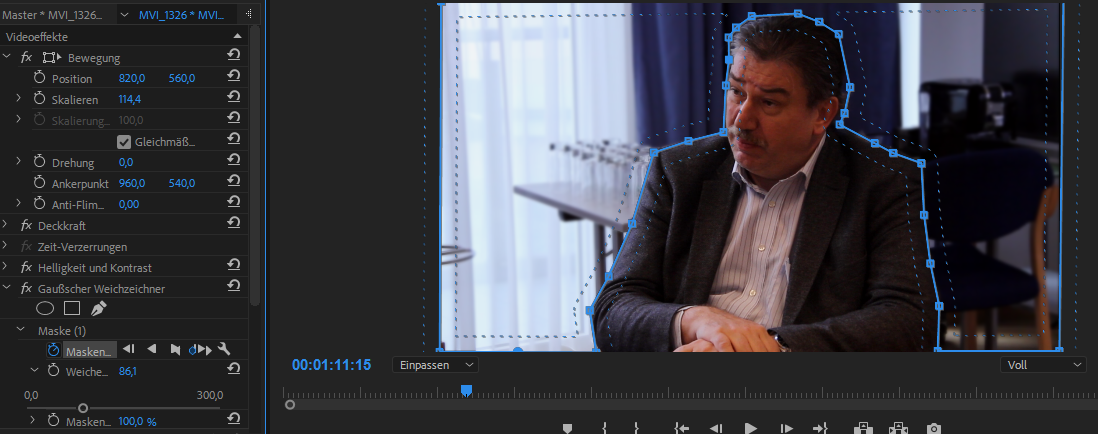
\includegraphics[width=1.0\textwidth]{abb28} 
	\caption{Maskenpfad des Interviews mit dem Abteilungsvorstand}\label{fig:abb28}
\end{figure}
\subsection{Geschwindigkeitseffekte}
Am Tag der offenen Tür wurde der Eingangsbereich der Schule für etwa 20 Minuten gefilmt. Dieses Video wurde schließlich für das Tag der offenen Tür Video verwendet. Um den Zuschauer kein 20 Minuten langes Video anschauen zu lassen, wurde die Geschwindigkeit des Videos beschleunigt, und somit ein Zeitraffer erzeugt. Mit einem Rechtsklick auf die Spur kann man auch schon die Eigenschaft "Geschwindigkeit/Dauer" auswählen, bei der man die Geschwindigkeit beschleunigen oder verlangsamen kann.\footnote{vgl. Jörg Jovy, 2017, S. 475ff.}
\subsection{Musik}
Bei dem Tag der offenen Tür Video und dem Quiz wurde lizenzfreie Musik eingebunden. Diese stammt von Soundcloud. Die Verwendung von Musik lockert das Schauen eines Videos auf und löst beim Menschen Spannung, Mitleid, Angst oder Entspannung aus. Weiters dient die Musik geräuschlose Szenen zu überbrücken und sie so angenehmer machen.\footnote{vgl. Jörg Jovy, 2017, S. 365}
\subsection{Export}
Bei dem Export eines Videos in Adobe Premiere muss man sich zuerst für ein Format entscheiden, in dem man das Video exportieren möchte. Heutzutage wird der H.264 von allen Browsern unterstützt und deswegen wurden auch die Videos in dem Codec kodiert. Jedoch unterstützen veraltete Mozilla Firefox Browser keinen H.264 Codec, sondern den Web.m Codec. Um zu gewährleisten, dass sich jeder User die Videos ansehen kann, wurden die Videos auch im Web.m Codec kodiert. Da Adobe Premiere den Web.m Codec nicht implementiert hat, war es notwendig diesen mittels einer msi Datei einzubinden. \footnote{vgl. https://helgeklein.com/blog/2017/12/browser-video-codecs-formats-hardware-acceleration/ [Zugriff: 02.04.2018]}\footnote{vgl. https://www.soeren-hentzschel.at/firefox/mozilla-integriert-openh264-video-codec-von-cisco-in-firefox-33/ [Zugriff: 02.04.2018]}